%
% ME4140 - Fall 2016 - Fall 2020
% ROS by Tristan Hill - Tutorials for TnTech Students
% Virtualizing Ubuntu

\documentclass[12pt]{article}
\usepackage{hyperref}
\usepackage[pdftex]{graphicx}
\usepackage{multirow}
\usepackage{setspace}
\usepackage{color}
\usepackage{multicol}

\hypersetup{
    bookmarks=true,         % show bookmarks bar?
    unicode=false,          % non-Latin characters in Acrobat’s bookmarks
    pdftoolbar=true,        % show Acrobat’s toolbar?
    pdfmenubar=true,        % show Acrobat’s menu?
    pdffitwindow=false,     % window fit to page when opened
    pdfstartview={FitH},    % fits the width of the page to the window
    pdftitle={My title},    % title
    pdfauthor={Author},     % author
    pdfsubject={Subject},   % subject of the document
    pdfcreator={Creator},   % creator of the document
    pdfproducer={Producer}, % producer of the document
    pdfkeywords={keyword1, key2, key3}, % list of keywords
    pdfnewwindow=true,      % links in new PDF window
    colorlinks=true,       % false: boxed links; true: colored links
    linkcolor=red,          % color of internal links (change box color with linkbordercolor)
    citecolor=green,        % color of links to bibliography
    filecolor=magenta,      % color of file links
    urlcolor=blue           % color of external links
}

% custom colors
\definecolor{TTUpurple}{rgb}{0.3098, 0.1607, 0.5176} % TTU Purple (primary)
\definecolor{TTUgold}{rgb}{1.0000, 0.8666, 0.0000} % TTU Gold (primary) 
\definecolor{mygray}{rgb}{.6, .6, .6}
\definecolor{mypurple}{rgb}{0.6,0.1961,0.8}
\definecolor{mybrown}{rgb}{0.5451,0.2706,0.0745}
\definecolor{mygreen}{rgb}{0, .39, 0}
\definecolor{mypink}{rgb}{0.9960, 0, 0.9960}

% color commands
\newcommand{\R}{\color{red}}
\newcommand{\B}{\color{blue}}
\newcommand{\BR}{\color{mybrown}}
\newcommand{\K}{\color{black}}
\newcommand{\G}{\color{mygreen}}
\newcommand{\PR}{\color{mypurple}}
\newcommand{\PN}{\color{mypink}}
\newcommand{\OR}{\color{TTU}}
\newcommand{\GD}{\color{TTUgold}}

\newcommand{\Lagr}{\mathcal{L}} % lagrangian

\newcommand{\hspcu}{\underline{\hspace{20mm}}} % large horizontal space w underline
\newcommand{\vspccc}{\vspace{6mm}\\} % large vertical space
\newcommand{\vspcc}{\vspace{4mm}\\}   % medium vertical space
\newcommand{\vspc}{\vspace{2mm}\\}     % small vertical space

\newcommand{\hspcccc}{\hspace{10mm}} % large horizontal space
\newcommand{\hspccc}{\hspace{6mm}} % large horizontal space
\newcommand{\hspcc}{\hspace{4mm}}   % medium horizontal space
\newcommand{\hspc}{\hspace{2mm}}     % small horizontal space

\newsavebox{\mybox} % custom box

\textwidth=6.5in
\topmargin=-0.5in
\textheight=9.25in
\hoffset=-0.5in
\footskip=0.2in

\pagestyle{myheadings}
\markright{{\large ME 4140 Fall 2020---Virtualizing Ubuntu Linux with Virtual Box}}

\newcommand{\homeWeight}{10}
\newcommand{\quizWeight}{20}
\newcommand{\examWeight}{15}
\newcommand{\finalWeight}{25}

\begin{document}

\thispagestyle{plain}

\begin{center}
   {\bf \Large ROS - Virtualizing Ubuntu Linux with Virtual Box}\vspace{3mm} \\
   {\bf \large ME 4140 - Introduction to Robotics - Fall 2020} \vspace{5mm}\\
\end{center}


\begin{description}

 	\item[What is a \href{https://en.wikipedia.org/wiki/Virtual_machine}{Virtual Machine} ?]: \\
 	\begin{multicols}{2}
      		
            \begin{itemize}
                
                \item A virtual machine is an operating system that is installed or {\it virtualized} inside another operating system.
                \item This is useful for learning and testing, but it is resource intensive and is not ideal for permanent use. 
                \item \href{https://www.virtualbox.org/}{VirtualBox} is a trusted application commonly used for this process
                
            \end{itemize}
            
\includegraphics[scale=.15]{CaptureA.png}\\
	\end{multicols}
	
	\item[Overview of Setup Process]: \vspace{0mm} \\

		        First you will download and install VirtualBox from Oracle which is an application for {\it virtualizing} operating systems on top of an existing one. Next you will download the Ubuntu installation .iso file and setup a virtual operating system for learning ROS. This requires a large file that I recommend downloading ahead of time. Finally, you will be ready to install the ROS Melodic software package in Ubuntu which is described in detailed in the next module. 

	\item[System Requirements]: \vspace{0mm} \\

		        \begin{itemize}

					\item {\bf CPU:} Most modern notebook or desktop computers will work well. If you are using a very old computer it may be very slow. A tablet or Chromebook is not supported.
					\item {\bf Memory:} At least 8Gb of RAM is recommended.        
               
                    \item {\bf Storage:} You need approximately 20Gb of free space on a hard drive to install your virtual operating system. This space will remain in its current partition and you are free to delete the files when you are finished. USB 2.0 or slower connection to the hard drive is not recommended. 
    
                \end{itemize}
			\item[Disclaimer]: \begin{itemize}
			\item {\bf \R It is a good idea to back up any important files before you begin a project.} 
			\item Some students may have to adjust a computer BIOS setting to allow virtualization. This setting can be easily reverted.   
			\item It is recommended to have your computer's power supply available before you begin this installation process. 
			\end{itemize} 			
			
			
                    
  

\newpage

\item[Detailed Setup Process ]: \vspace{0mm} \\

	\begin{enumerate} 
	
	
	
	
\item Install VirtualBox Application: \\

\begin{enumerate} 
	
\item Download the VirtualBox installation file from ilearn. Choose the file that matches your computer type. If you are using a Linux computer already, skip step 1 and proceed to step 2. \vspace{5mm}

\item Click the VirtualBox installation file you downloaded and install the application. You will need to provide admistrator access and click allow. You no longer need the installation file, but it is small so it wont hurt to keep it. \vspace{5mm} \\

\end{enumerate}
  
\item Install Virtual Operating System: \vspace{0mm} \\
\begin{enumerate} 
    	\item Open the VirtualBox application you installed in step 2. \vspace{5mm} \\
      		\hspace*{-2.5cm}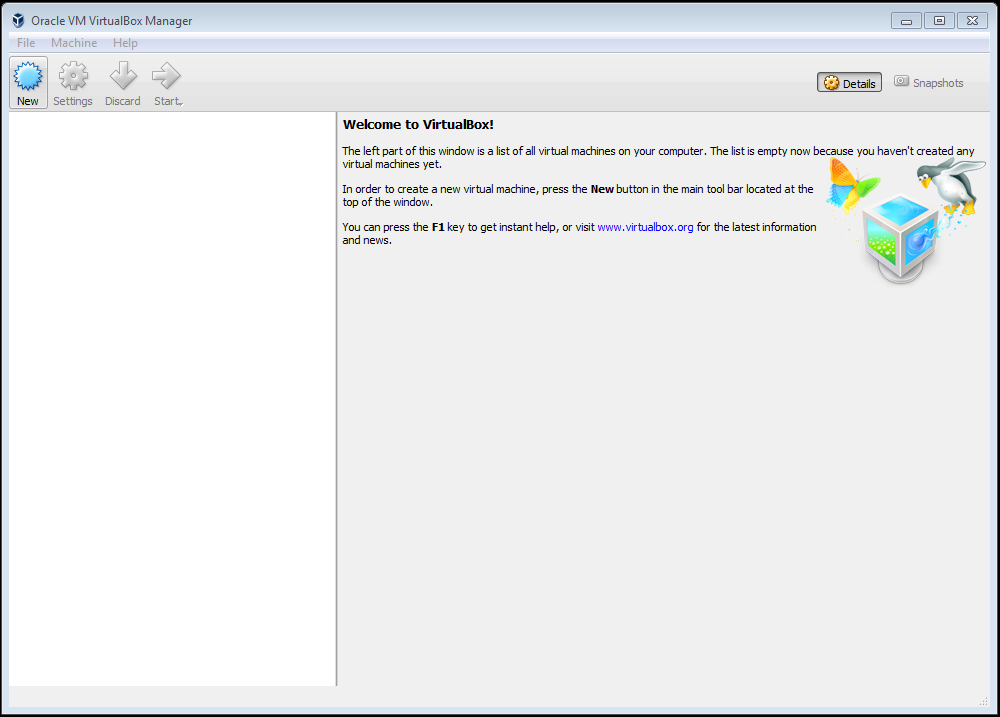
\includegraphics[scale=.6]{Capture1.png}\\
            \begin{itemize}
                
                \item before proceeding make sure you have an {\bf \B internet connection }
                \item before proceeding make sure you have access to a {\bf \R power supply or battery }
                
            \end{itemize}
            
            \end{enumerate}
	\newpage
	\item Create New Virtual Machine: \vspace{20mm} \\
      		\hspace*{-2.5cm}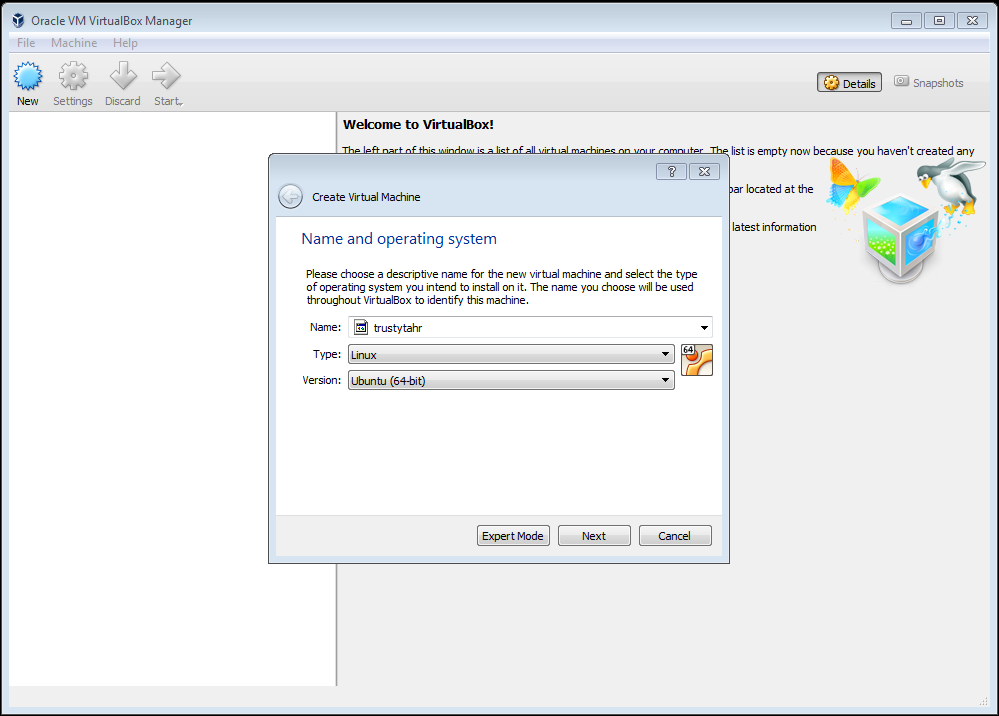
\includegraphics[scale=.6]{Capture2.png}\\
               \begin{itemize}
                
	\item press the {\bf new} button
                \item choose a {\bf computer name} (this is your choice but remember it!)
                \item choose an {\bf operating system} type (Linux)
                \item choose a {\bf version}, this depends on your physical machine This is probably Ubuntu 64-bit but possbily Ubuntu 32-bit) 
                
            \end{itemize}
	\newpage
\item Define Virtual Machine Parameters: \vspace{20mm} \\
      		\hspace*{-2.5cm}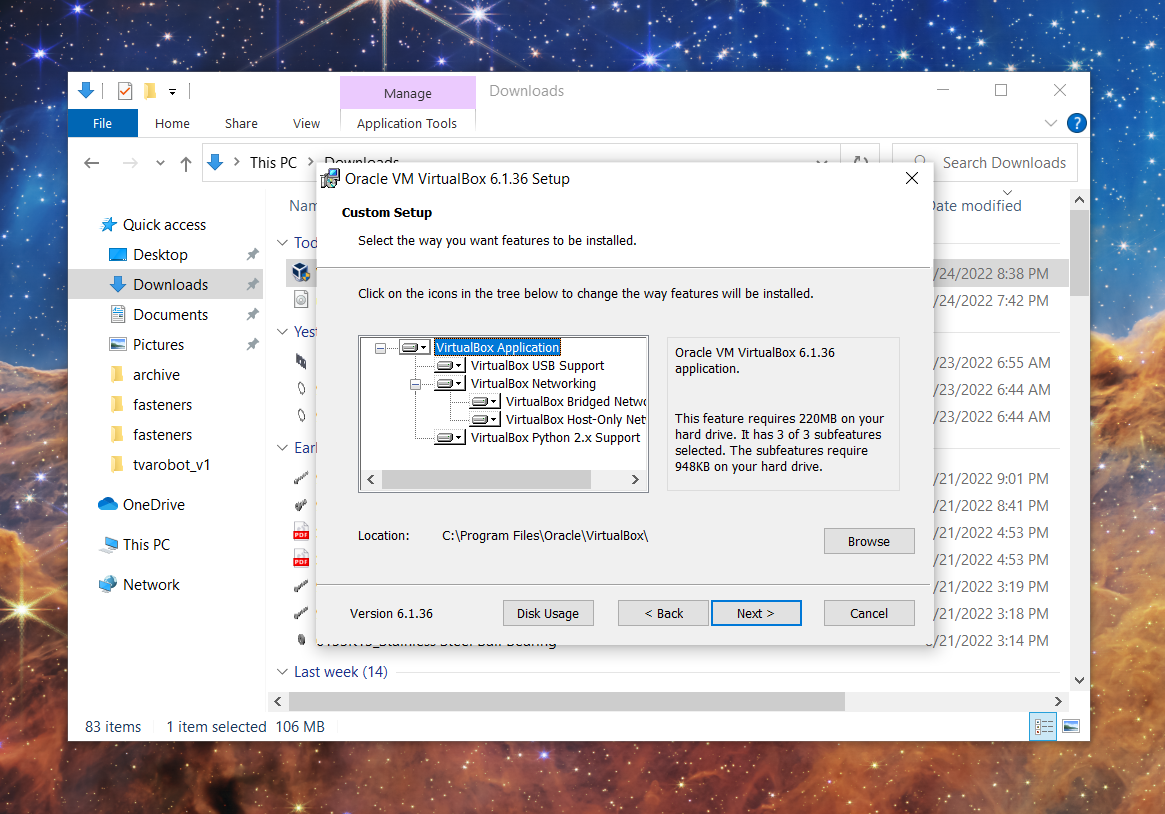
\includegraphics[scale=.6]{Capture3.png}\\
            \begin{itemize}
                
                \item Choose the amount of RAM you want to allocate to the VM
                \item This number is based on your available resources. More is better but it helps to leave some for windows. If your computer has 8GB total I suggest no more than 6GB for for VM.  
                
            \end{itemize}
	\newpage
\item Define Virtual Hard Drive Parameters: \vspace{20mm} \\
      		\hspace*{-2.5cm}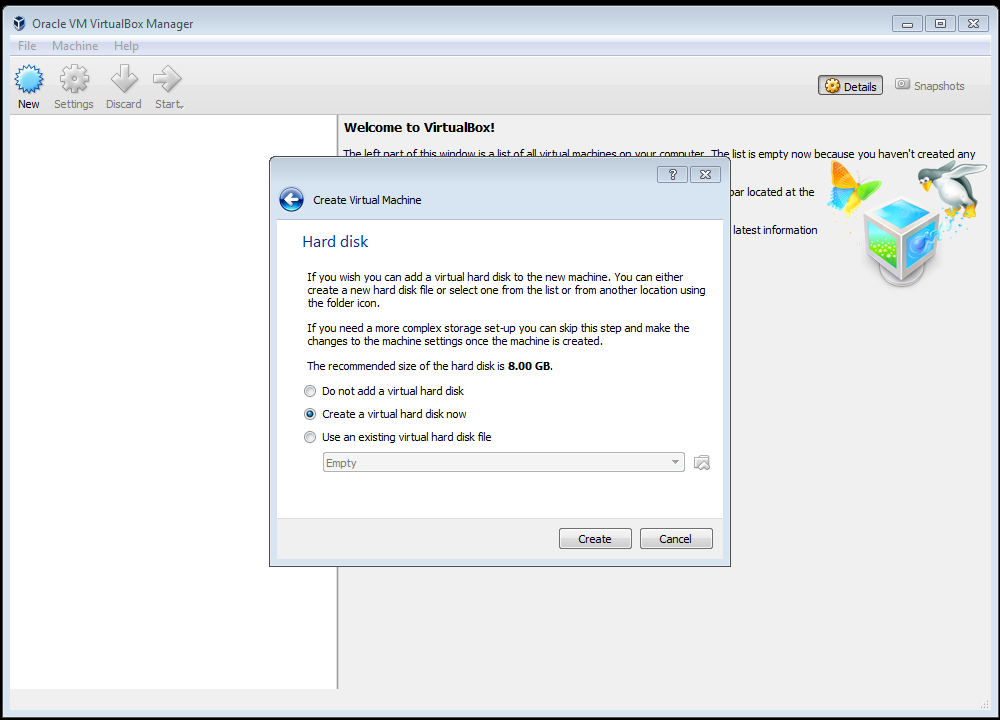
\includegraphics[scale=.6]{Capture4.png}\\
 \begin{itemize}
                
                \item You must have enough space on your hard drive to virutalize linux and install ros. 
                \item {\bf create a virtual hard drive now}
                
            \end{itemize}
	\newpage
\item Virtual Hard Drive Setup: \vspace{20mm} \\
      		\hspace*{-2.5cm}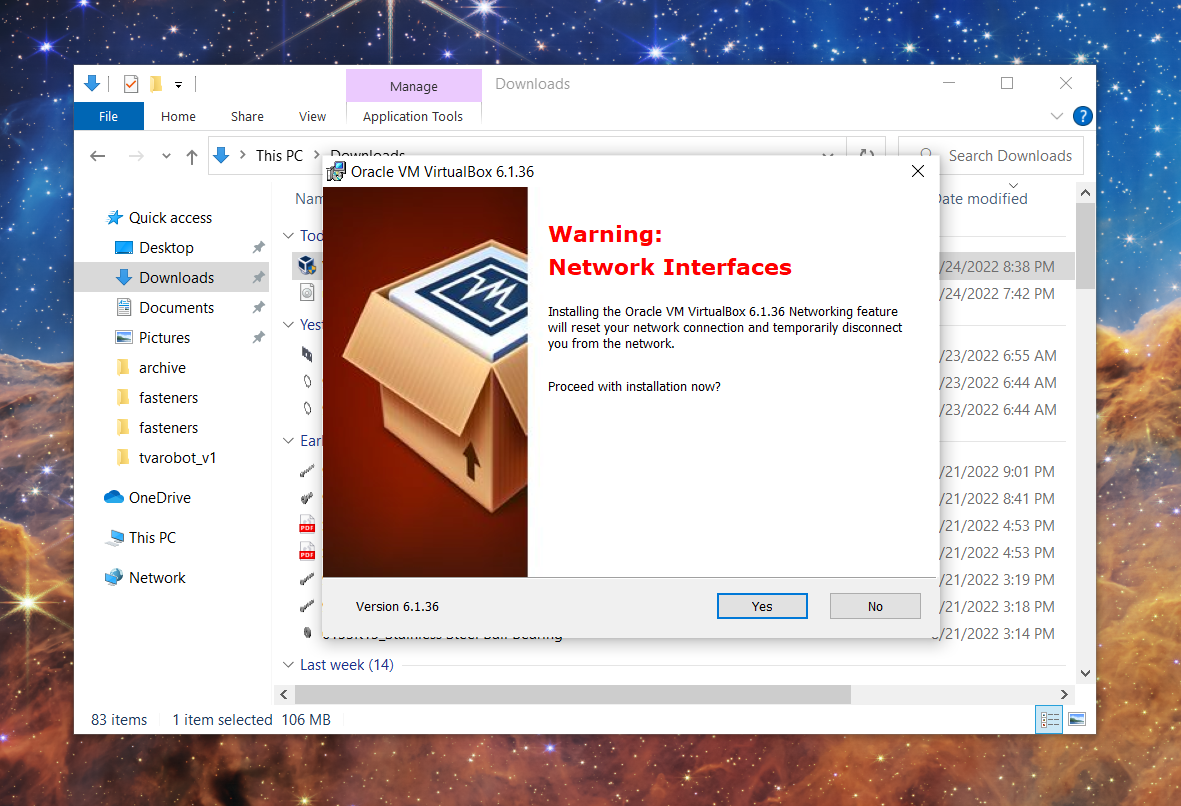
\includegraphics[scale=.6]{Capture5.png}\\
            \begin{itemize}
                
                \item Create a {\bf fixed size} virtual hard drive. 
                              
            \end{itemize}
	\newpage
\item Virtual Hard Drive Setup: \vspace{20mm} \\
        \hspace*{-2.5cm}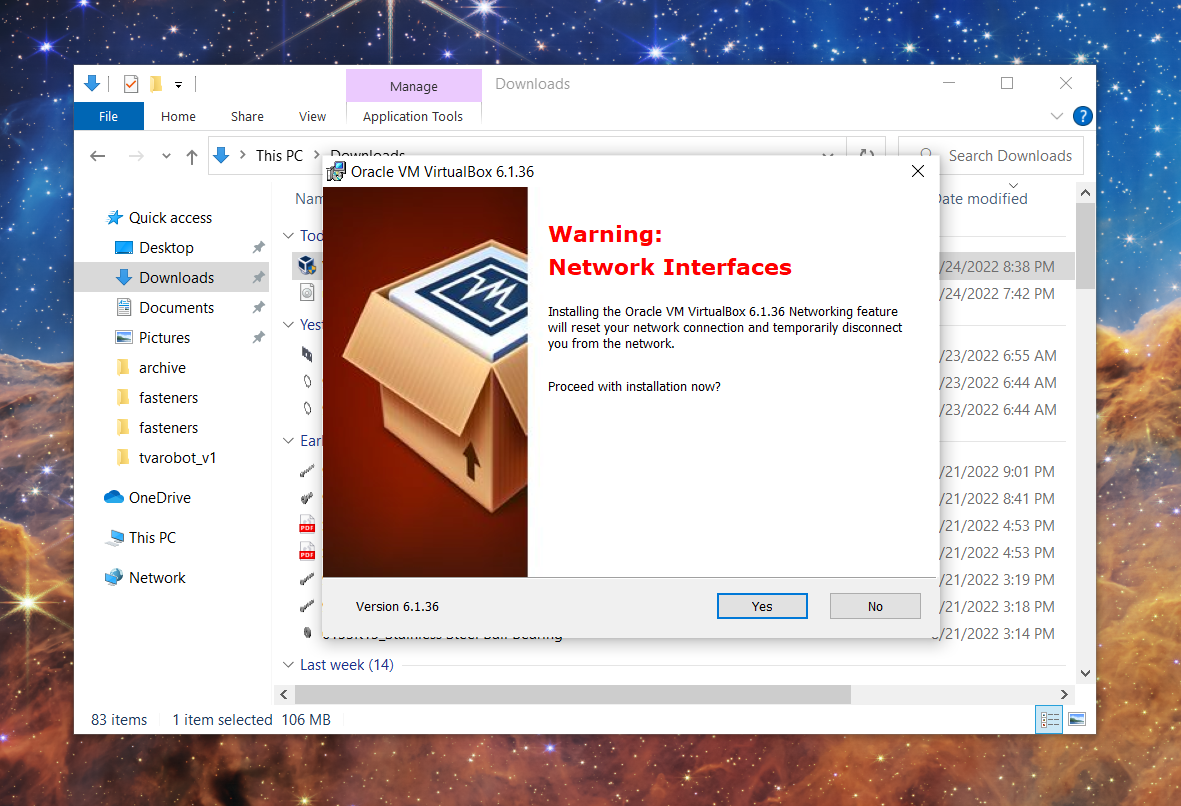
\includegraphics[scale=.6]{Capture5.png}\\
        \begin{itemize}
                        
                \item Choose the virtual hard drive type. 
                \item VDI is recommended.
                           
        \end{itemize}
\newpage
\item Virtual Hard Drive Setup : \vspace{20mm} \\
      		\hspace*{-2.5cm}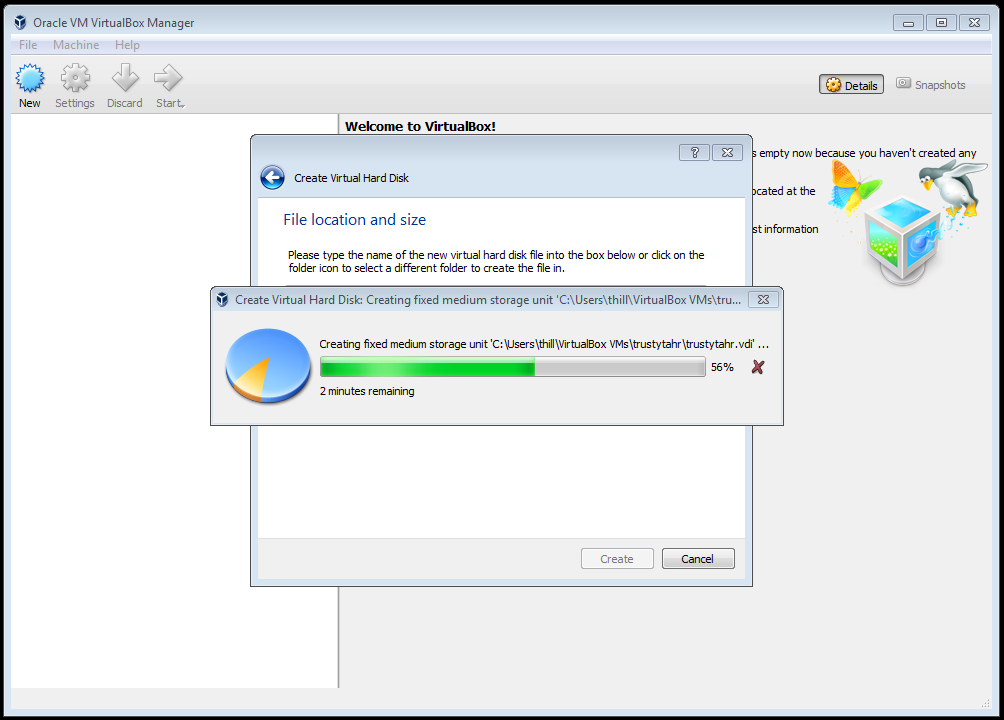
\includegraphics[scale=.6]{Capture6.png}\\
             \begin{itemize}
                    
                \item choose the size of your virtual hard drive       
                \item to virtualize Ubuntu and install ROS it is recommended to make a 16 GB VDI
                \item  you can experiment with 'lighter versions' 
          
                    \begin{itemize}
                            
                        \item lubuntu     
                        \item many more
                        \item I am working on this
                        
                    \end{itemize}
                
            \end{itemize}
	\newpage

\end{enumerate}

		\item[Ubuntu OS Installation and Setup]: \vspace{20mm} \\

\begin{enumerate}
\item Start the VM for the first time: \vspace{20mm} \\
      		\hspace*{-2.5cm}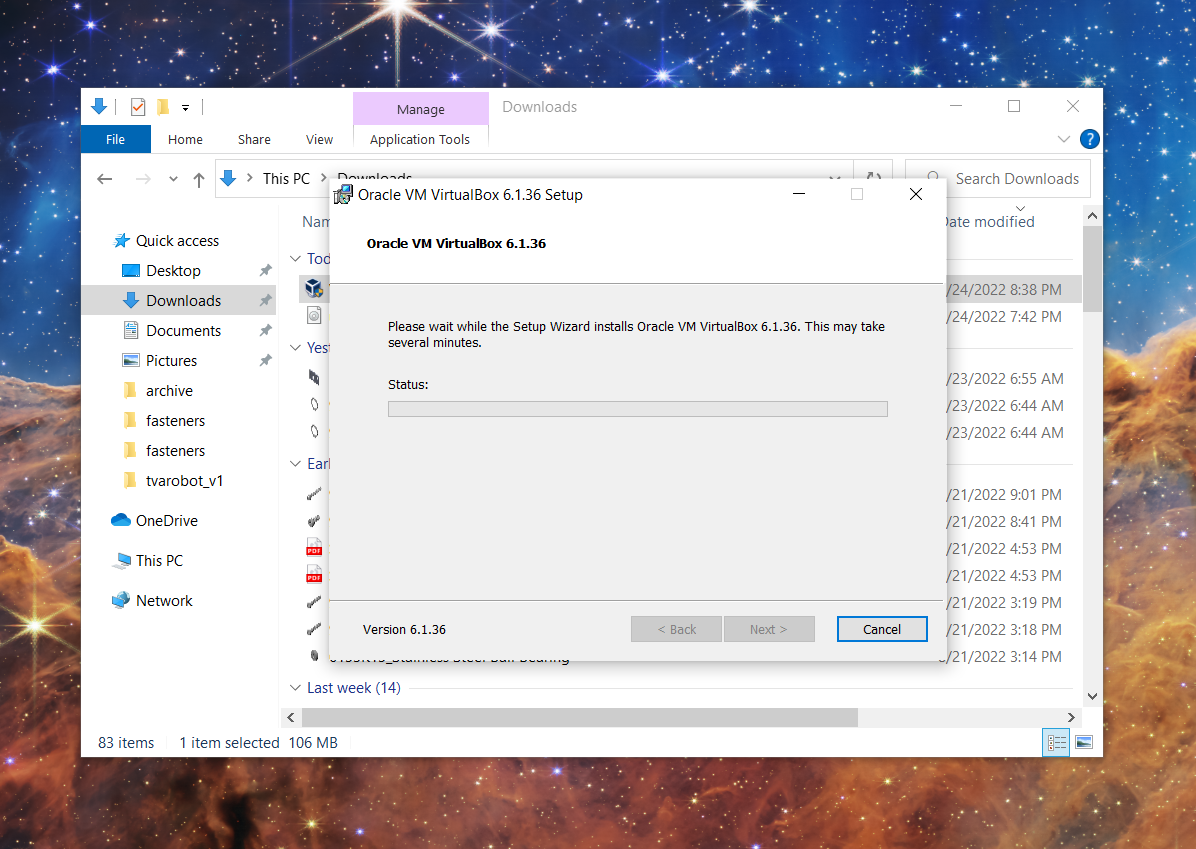
\includegraphics[scale=.6]{Capture7.png}\\
            \begin{itemize}
                    
                 \item select your newly created VM      
                 \item press the green start button
                 \item wait for it...       
            \end{itemize}
	\newpage
\item Start the VM for the first time: \vspace{20mm} \\
      		\hspace*{-2.5cm}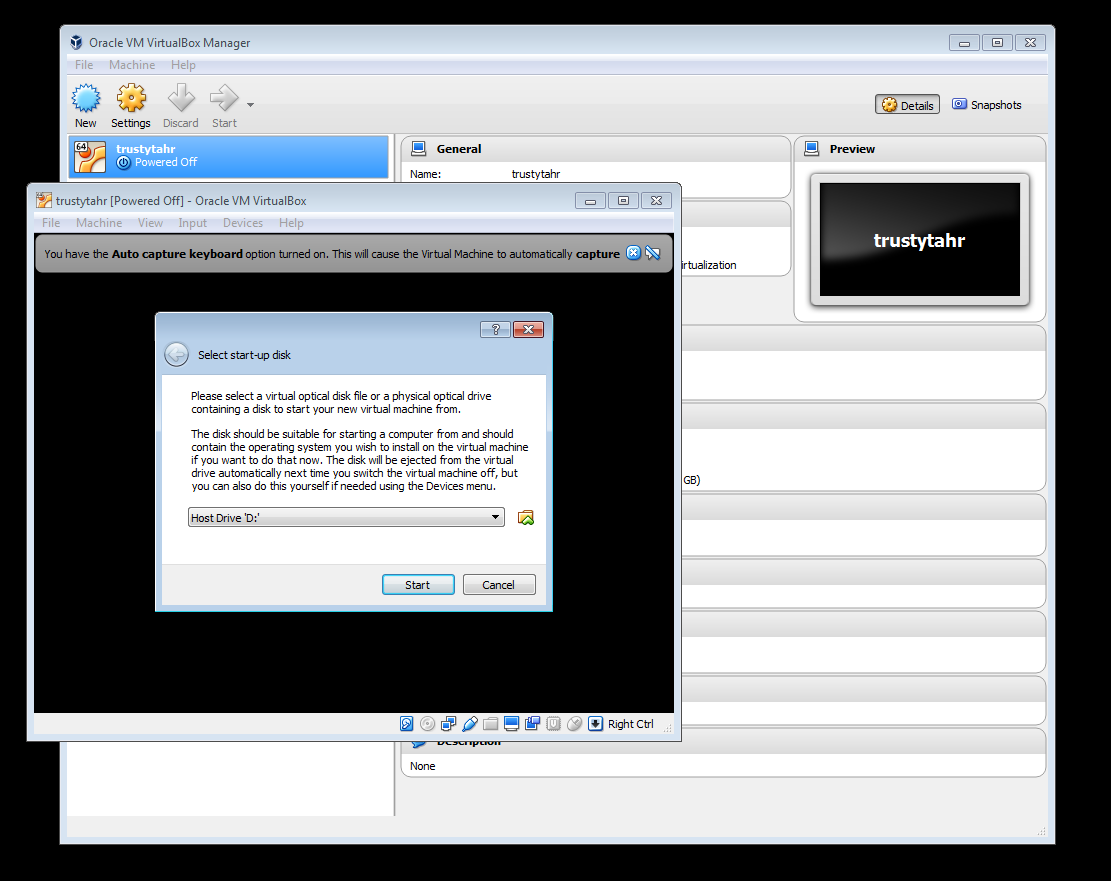
\includegraphics[scale=.6]{Capture8.png}\\
            \begin{itemize}
                    
                 \item choose to select media from a local folder 
                 \item wait for it...
                 
            \end{itemize}
	
\item Start the VM for the first time: \vspace{20mm} \\
      		\hspace*{-2.5cm}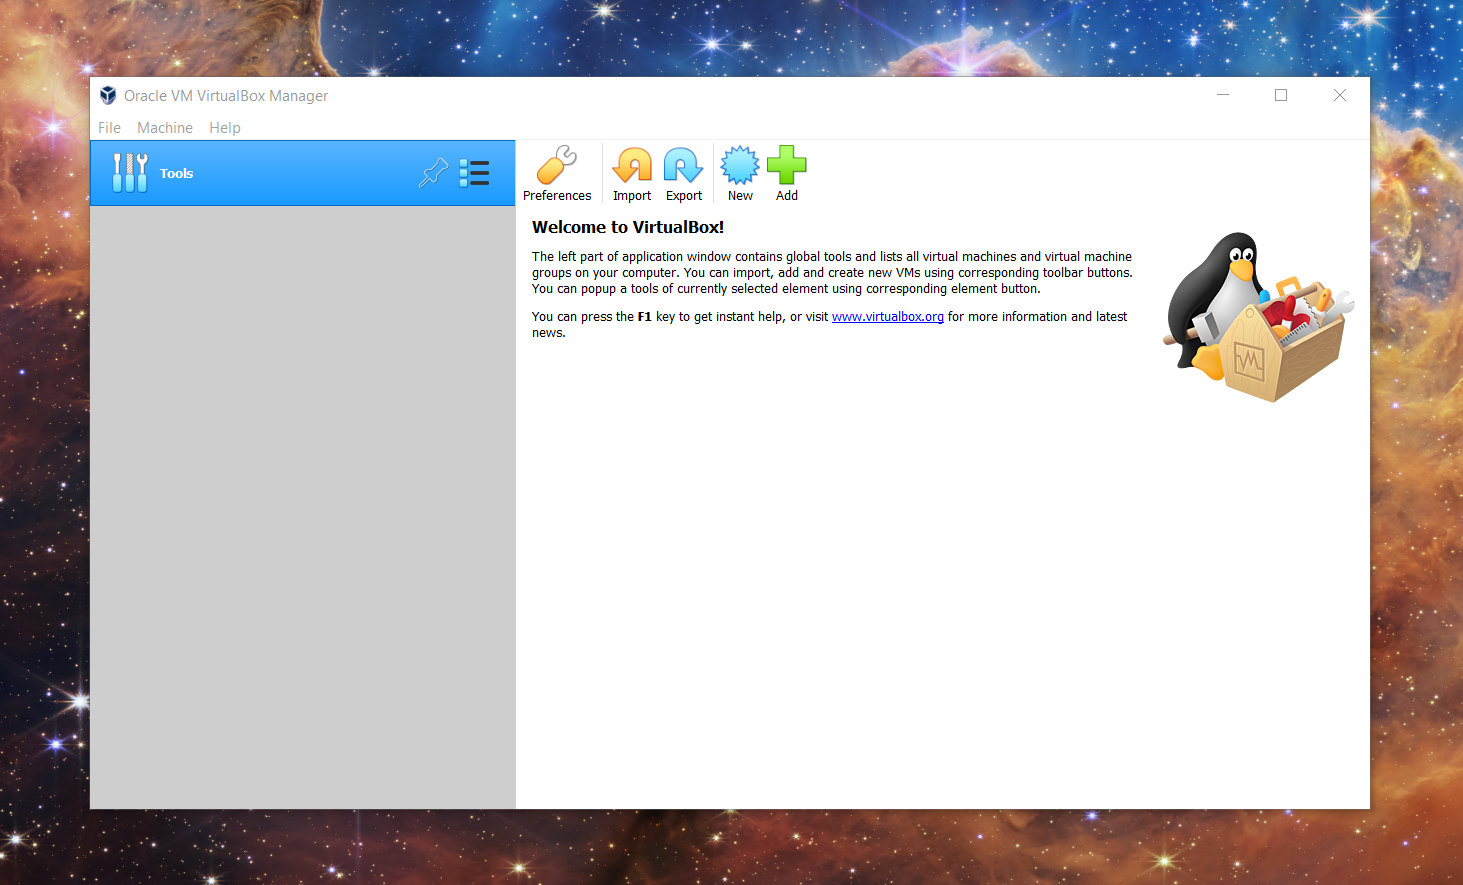
\includegraphics[scale=.6]{Capture9.png} \\
               \begin{itemize}
                    
     
                \item choose the Ubuntu .iso file that you aquired
                \item it is recommended that the media is on the local machine
                \item wait for it...
                
            \end{itemize}


        
	\newpage
\item Ubuntu Installation: \vspace{20mm} \\
      		\hspace*{-2.5cm}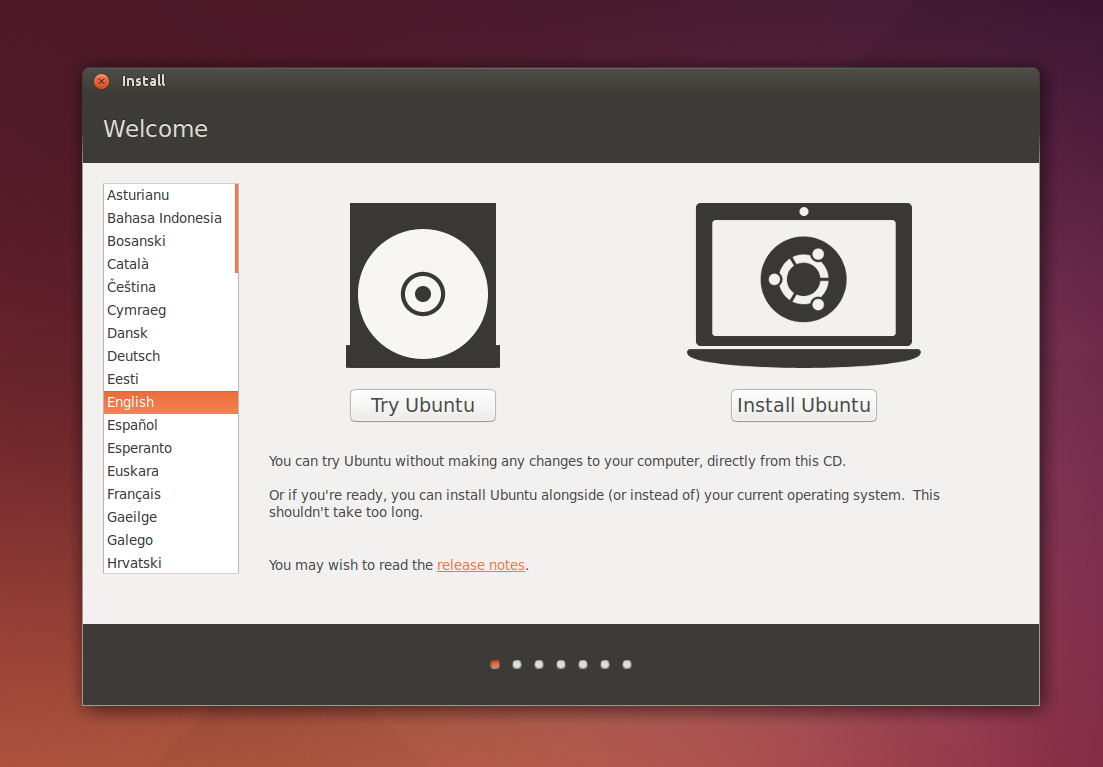
\includegraphics[scale=.6]{Capture10.png}
            \begin{itemize}
                    
                 \item {\bf Install Ubuntu} (harmless if using VirtualBox)
                 \item try is just temporary (single session)
                 \item wait for it...    
            \end{itemize}
	\newpage
\item Ubuntu Installation: \vspace{20mm} \\
      		\hspace*{-2.5cm}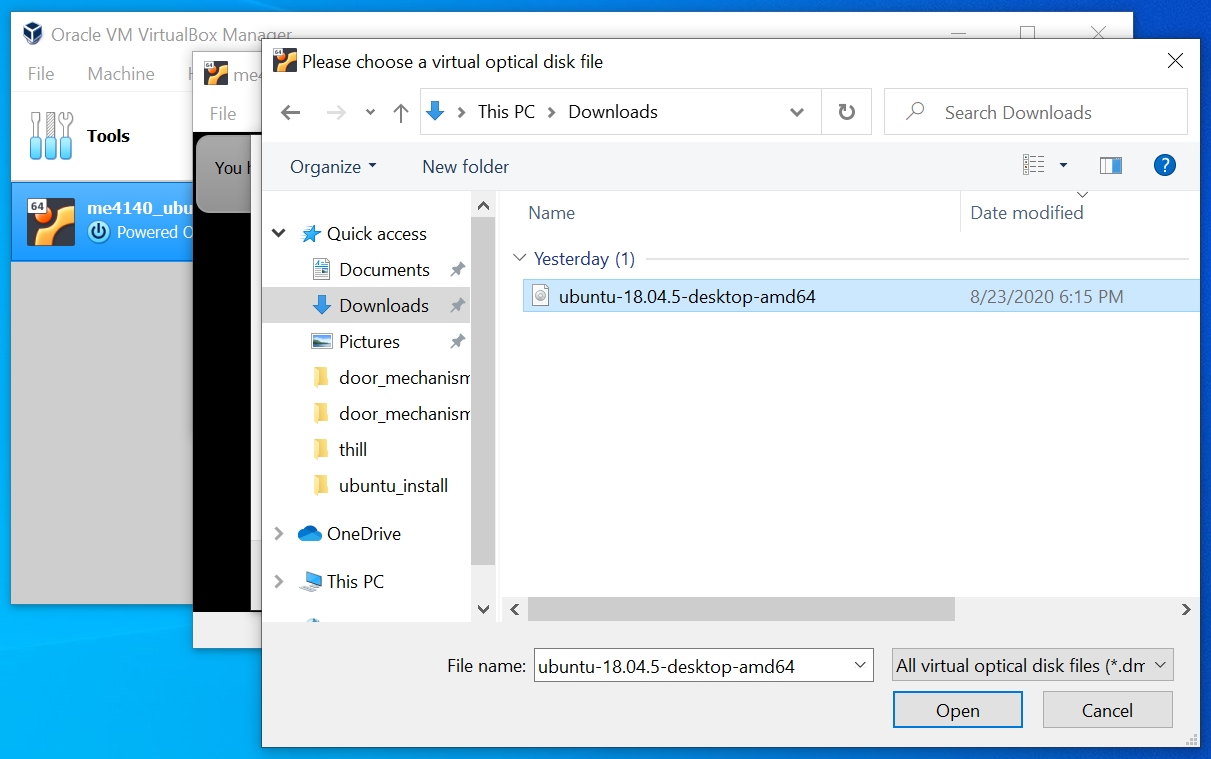
\includegraphics[scale=.6]{Capture11.png} 
            \begin{itemize}
                    \item check that you meet the requirements
                 \item click the two check boxes for proprietary drivers
            \end{itemize}
	\newpage
\item Ubuntu Installation: \vspace{20mm} \\
      		\hspace*{-2.5cm}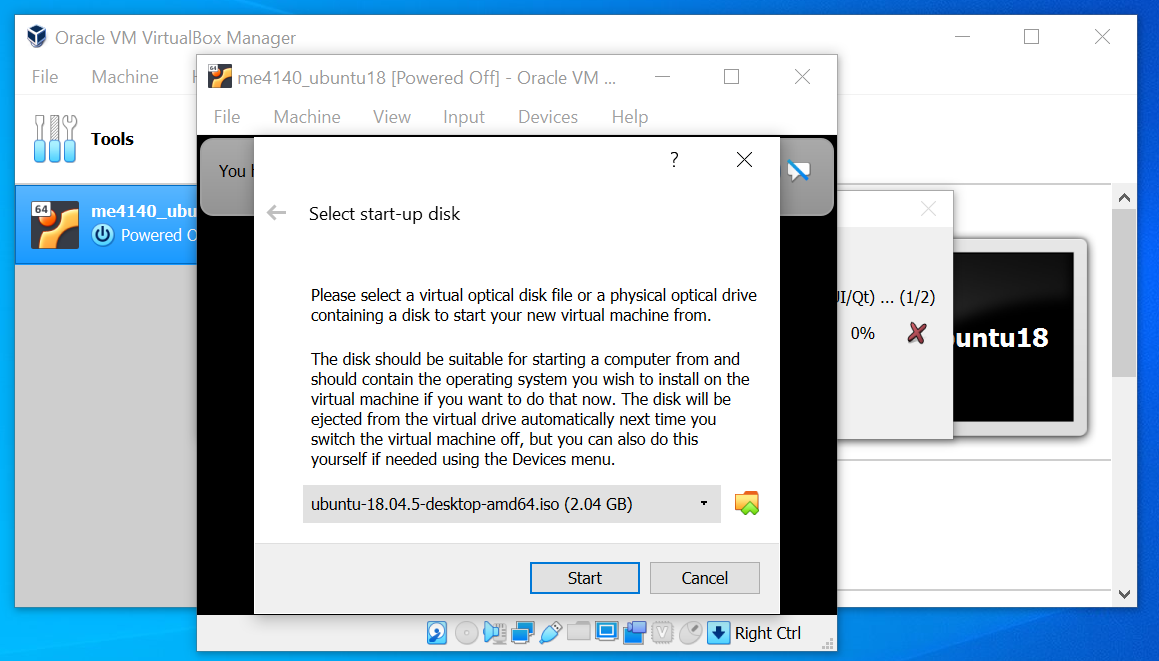
\includegraphics[scale=.6]{Capture12.png}\\
             \begin{itemize}
                    
                 \item {\bf Erase Everything and Install Ubuntu} (harmless if using VirtualBox)
                 \item DANGEROUS AND PERMANENT IF NOT USING VIRTUALBOX
                 \item wait for it...    
            \end{itemize}
	\newpage
\item Wait Wait Wait: \vspace{20mm} \\
      		\hspace*{-2.5cm}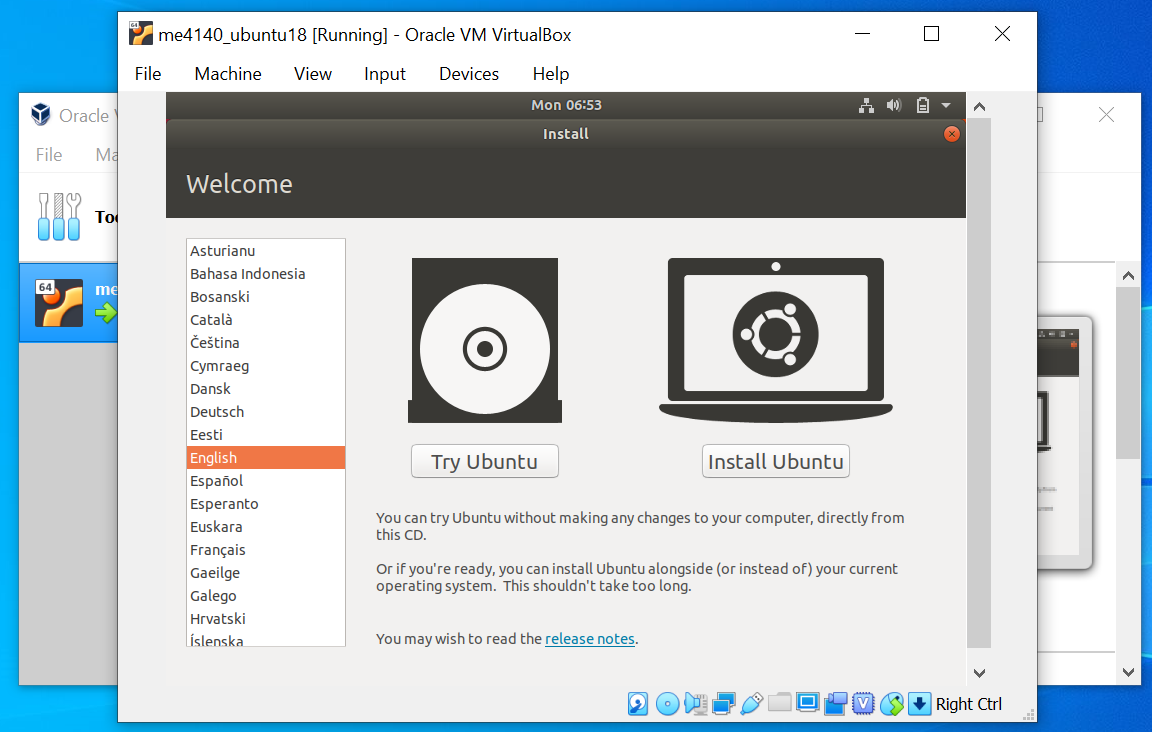
\includegraphics[scale=.6]{Capture13.png}
	\newpage
\item Shut Down The VM: \vspace{20mm} \\
      		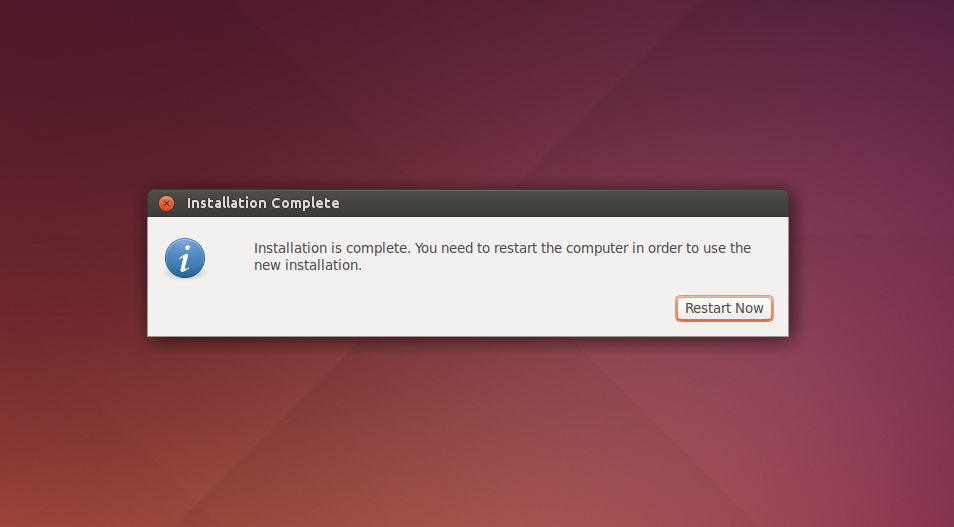
\includegraphics[scale=.6]{Capture14.png}\\
			
	\newpage
\item Shut Down The VM: \vspace{20mm} \\
      		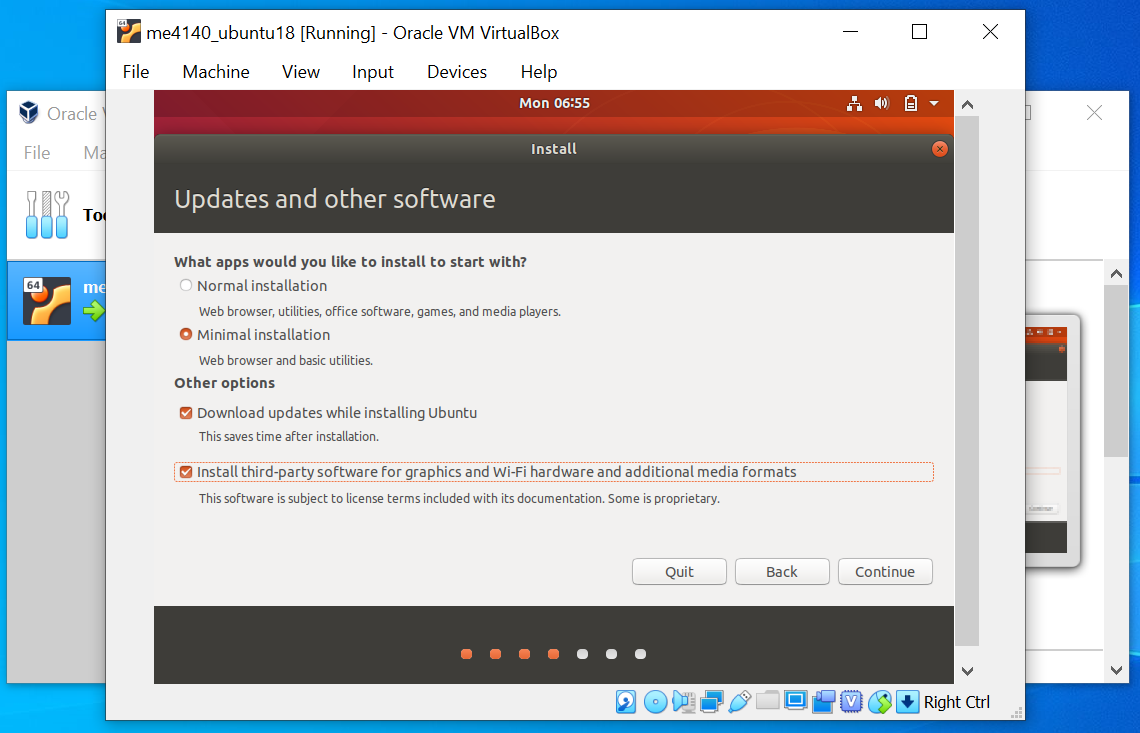
\includegraphics[scale=.6]{Capture15.png}
			\begin{itemize}
                 
				 \item wait for it...
                 \item after waiting a few moments you may have to close the window of the VM
                     
            \end{itemize}
	\newpage
\item Finally!: \vspace{20mm} \\
      		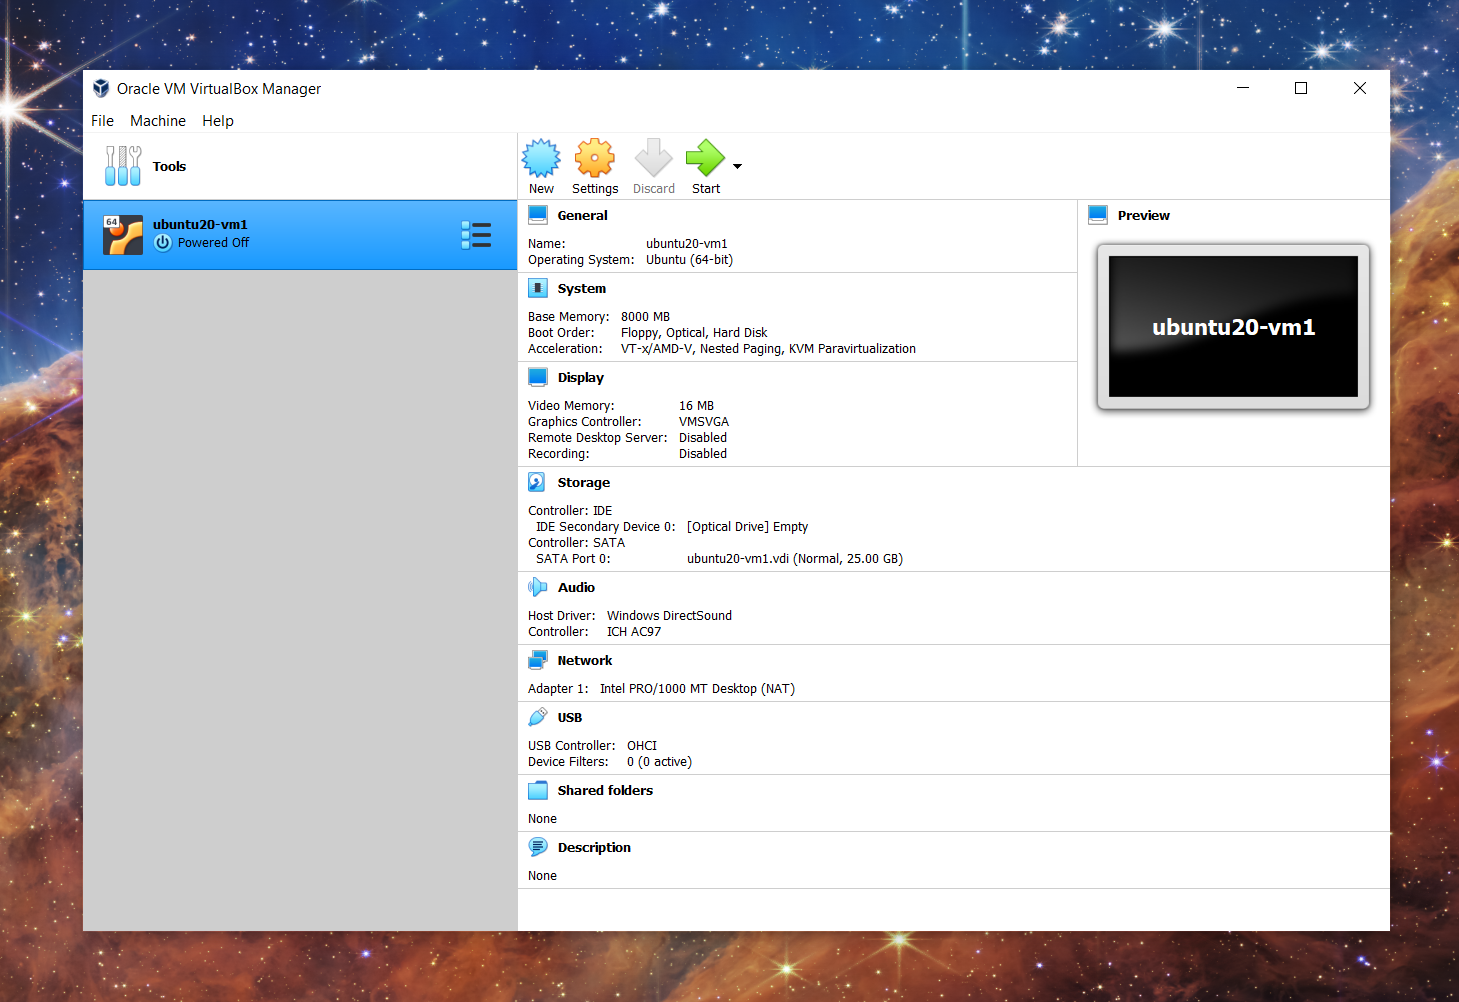
\includegraphics[scale=.6]{Capture16.png}
            \begin{itemize}
        \item POWER OFF the Machine
    \end{itemize} 
	\newpage
\item Now restart the VM!!!:
    \begin{itemize}
        \item the VM you made should be in the left list
        \item select it and click start
		\item the Ubuntu OS should appear	
    \end{itemize}        

\end{enumerate}    
\end{description}
\end{document}

